% D.26 相交弦：⊙O 中 AB、CD 交于 P
\documentclass[tikz,border=4pt]{standalone}
\usepackage{ctex}
\usepackage{amsmath}
\usetikzlibrary{calc}
\begin{document}
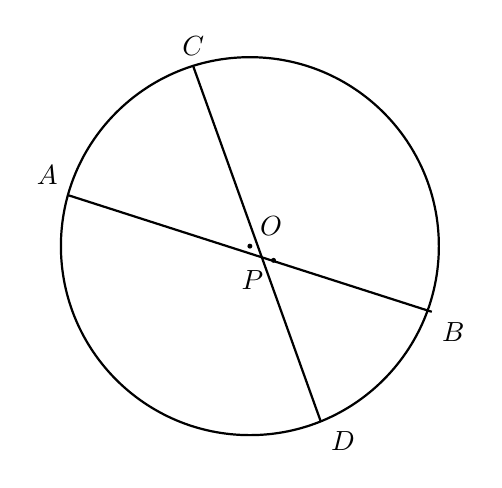
\begin{tikzpicture}[scale=0.6, thick]
  \coordinate (O) at (0, 0);
  \draw (O) circle (4);
  \coordinate (A) at (-3.5, 1.94);
  \coordinate (B) at ( 3.5,-1.94);
  \coordinate (C) at (-1.5, 3.71);
  \coordinate (D) at ( 1.5,-3.71);
  \coordinate (P) at (0, 0);  % 取过原点的弦交于 O 为简化（实际不一定过 O，仅示意）
  % 改为通用：让 P 不在中心
  \coordinate (P) at (0.5, -0.3);
  \coordinate (A) at (-3.85, 1.08);
  \coordinate (B) at ( 3.85, -1.39);
  \coordinate (C) at (-1.2,  3.81);
  \coordinate (D) at ( 1.5, -3.71);

  \draw (A) -- (B);
  \draw (C) -- (D);
  \fill (O) circle (1.5pt);
  \fill (P) circle (1.5pt);
  \node[above right] at (O) {$O$};
  \node[above left]  at (A) {$A$};
  \node[below right] at (B) {$B$};
  \node[above]       at (C) {$C$};
  \node[below right] at (D) {$D$};
  \node[below left]  at (P) {$P$};
\end{tikzpicture}
\end{document}
